\documentclass{article}
\usepackage{iclr2026_conference,times}
\input{math_commands.tex}
\usepackage{hyperref}
\usepackage{url}
\usepackage{xcolor}
\usepackage{graphicx}
\usepackage{booktabs}
\usepackage{subcaption}
\usepackage{multirow}

\newcommand{\TODO}[1]{{\color{red}\textbf{[TODO: #1]}}}

\title{Improving the Pretraining Efficiency of Diffusion Language Models}

\author{Chang-Han Chen \\
University of California, Berkeley\\
Berkeley, CA 94720, USA \\
\texttt{changhanc@berkeley.edu}
}

\iclrfinalcopy
\begin{document}
\maketitle

\begin{abstract}
Diffusion language models (dLMs) are slow to train but can eventually surpass autoregressive (AR) models in the data-constrained setting. Can we accelerate the crossover point at which dLMs win? We already found some interesting results about curriculum pretraining at 1M scale on TinyShakespeare and 50M scale on NVIDIA's ClimbMix, and outline upcoming data-constrained scaling experiments at 50M--300M. We suspect that the curriculum for optimal perplexity would be mostly AR, but the curriculum for optimal downstream performance would be more diffusion-heavy.
\end{abstract}

%=============================================================================
\section{Introduction}
\label{sec:intro}
%=============================================================================

The slogan is that "Diffusion models are super data learners" \citet{ni2025diffusionlanguagemodelssuper}: when unique training data is limited, the optimal performance of diffusion language models (dLMs) on downstream tasks can surpass autoregressive (AR) models. For example, a 1B-parameter dLM achieves over 56\% on HellaSwag using only 1B unique tokens. In fact, we are very likely moving toward an era where pretraining is more constrained by data than compute. 

But the reality is that dLMs remain substantially less compute-efficient to pretrain than AR models. Masked diffusion (MDLM) is roughly $14\times$ less efficient than AR per training token; uniform-noise diffusion is even worse, roughly $32\times$ less efficient. This is intuitive because any-order progressive decoding is a strictly harder task than autoregressive left-to-right generation.

If one really believes that dLMs are super data learners, then the top, if not only, priority should be to increase their compute efficiency.
There have been numerous works on A2D conversion \citep{efficientdlm2025, nbdiff2025, llada2_2025, sdar2025}. However, they all start with off-the-shelf, pretrained LLMs such as LLaMA or Qwen. Although this is convenient for getting strong benchmark results for the final model, it does not address the fundamental problem of how to improve the efficiency of dLM pretraining.

In this work, we study A2D conversion as a pretraining paradigm from
scratch, not (necessarily) as continual pretraining from off-the-shelf LLMs. In fact, the traditional A2D conversion becomes much more principled from this perspective: it is a special case of the \emph{curriculum pretraining} studied in our work, where the majority of the curriculum is next-token prediction.

This work is largely still in progress, mostly due to compute limitations. But we still present some interesting results: 1M-scale models on TinyShakespeare and a 50M model on NVIDIA's ClimbMix.

%=============================================================================
\section{Pilot Study: TinyShakespeare}
\label{sec:pilot}
%=============================================================================

We first validate the approach at small scale.  All models share a transformer
backbone with RoPE, QK-norm, ReGLU MLPs, and RMSNorm, spanning six sizes from
0.1M to 3M parameters.  We compare four diffusion objectives---MDLM,
Remasked, Edit-1, and Edit-2---each in standard and block (block length 4)
formulations.  We fix an IsoFLOP budget of $C = 6 \times 10^{14}$ and
determine training steps from the budget, model size, and per-step FLOP
multiplier ($6\times$ for standard, $12\times$ for block, $24\times$ for
block Edit-2). The details of these variants are not important because we find that they are not worth scaling up.

\textbf{AR warm-start has a U-shaped optimum at $p_{\mathrm{AR}} = 0.3$.}
We train AR for a fraction $p_{\mathrm{AR}}$ of total steps, then switch to
block MDLM.  Table~\ref{tab:pilot_curriculum} shows that $p_{\mathrm{AR}} =
0.3$ consistently gives the lowest validation loss: $-0.088$ nats at 0.3M and
$-0.077$ nats at 1M.  Too little AR undertrains the initialization; too much
starves the diffusion phase of training steps (Figure~\ref{fig:tiny}).

\begin{figure}[t]
    \centering
    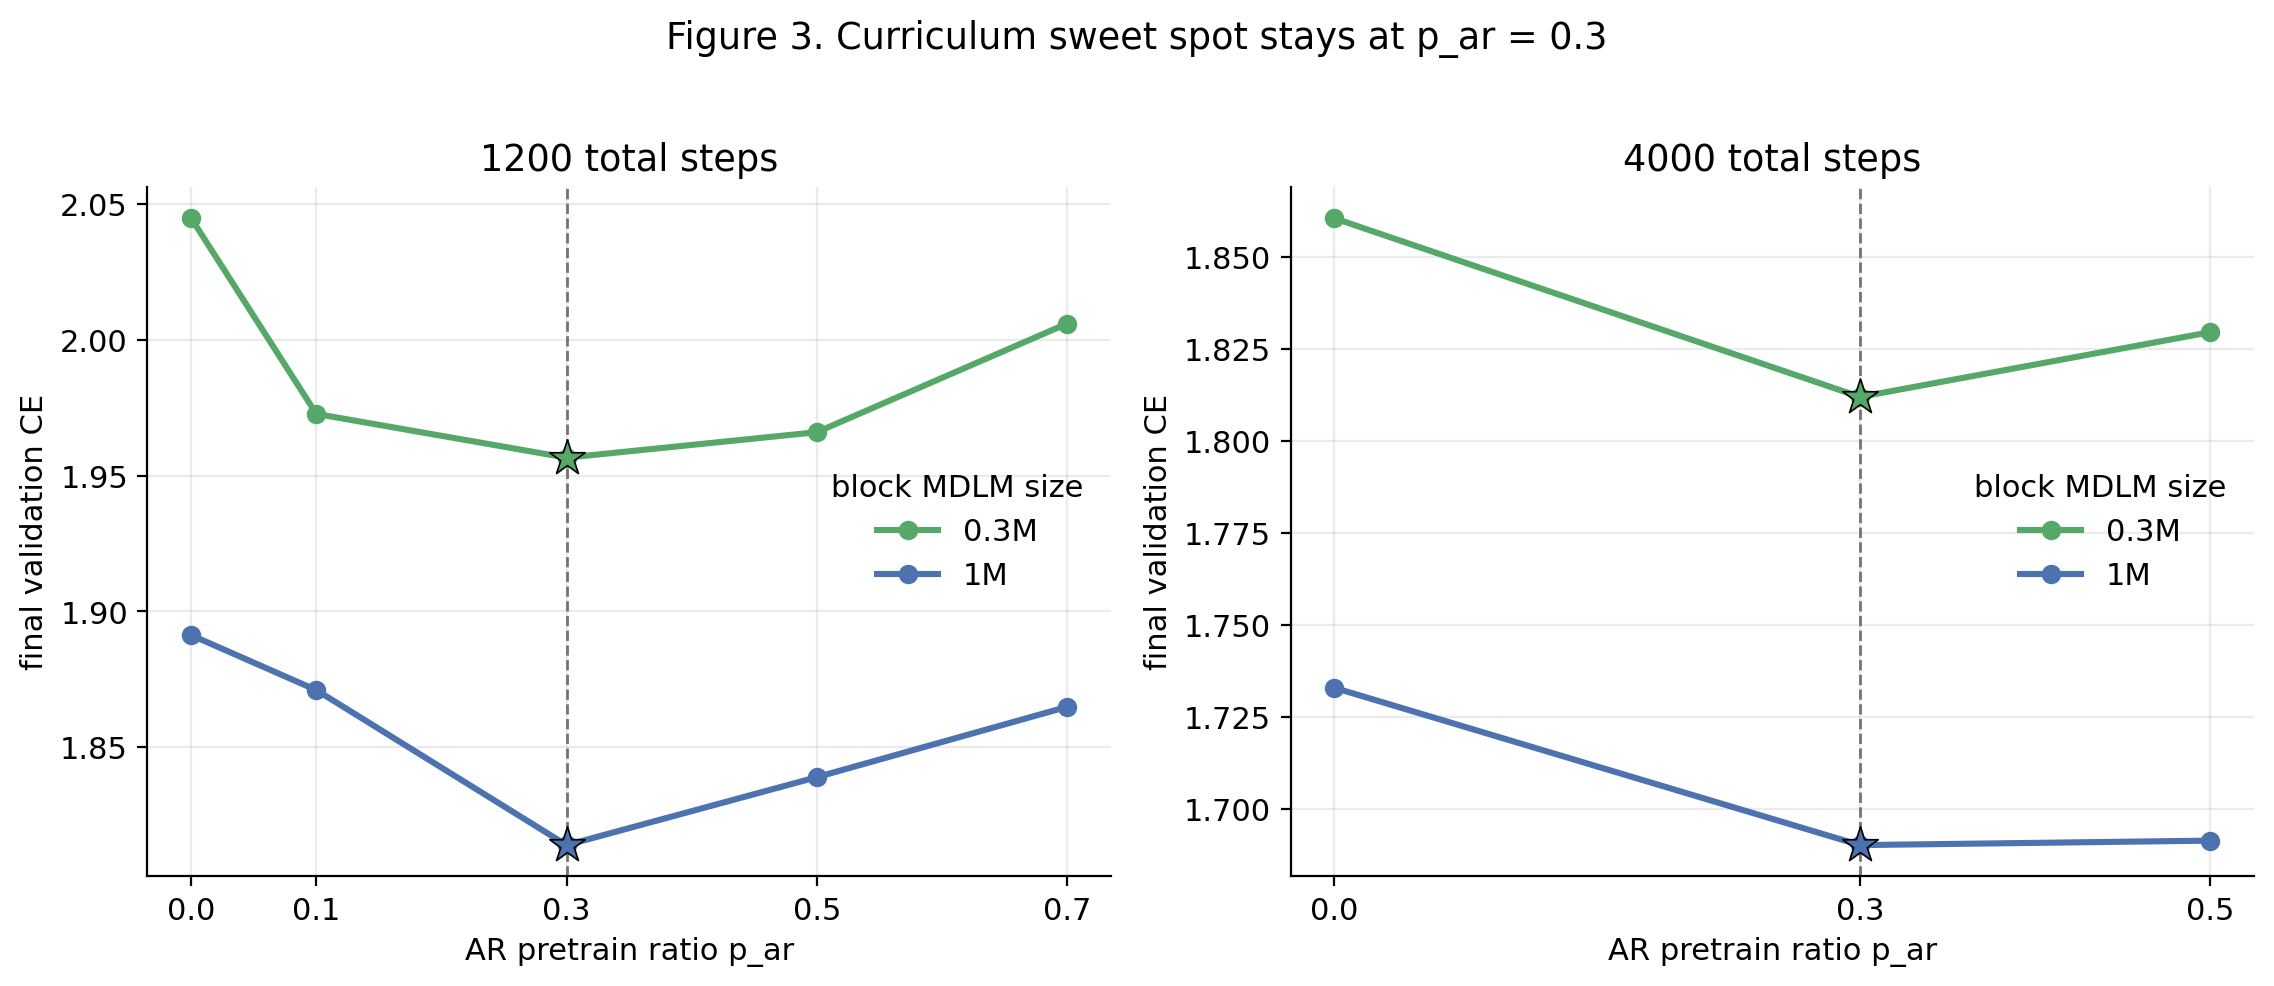
\includegraphics[width=0.5\linewidth]{figure3_curriculum_sweet_spot.png}
    \caption{30\% AR warmup is the most effective even when compute becomes $3$x (1200 to 4000 steps).}
    \label{fig:tiny}
\end{figure}

\begin{table}[t]
\centering
\caption{Pilot: validation CE for AR$\to$Block MDLM curriculum on
TinyShakespeare. Bold = best per row.}
\label{tab:pilot_curriculum}
\vspace{2pt}
\small
\begin{tabular}{lcccccl}
\toprule
& \multicolumn{5}{c}{1200 total steps} & \\
\cmidrule(lr){2-6}
Size & $p{=}0$ & $p{=}0.1$ & $p{=}0.3$ & $p{=}0.5$ & $p{=}0.7$ & $\Delta$ \\
\midrule
0.3M & 2.045 & 1.973 & \textbf{1.957} & 1.966 & 2.006 & $-$0.088 \\
1M   & 1.891 & 1.871 & \textbf{1.814} & 1.839 & 1.865 & $-$0.077 \\
\midrule
& \multicolumn{3}{c}{4000 total steps} & & & \\
\cmidrule(lr){2-4}
Size & $p{=}0$ & $p{=}0.3$ & $p{=}0.5$ & & & $\Delta$ \\
\midrule
0.3M & 1.860 & \textbf{1.812} & 1.830 & & & $-$0.049 \\
1M   & 1.733 & \textbf{1.690} & 1.692 & & & $-$0.043 \\
\bottomrule
\end{tabular}
\vspace{-8pt}
\end{table}


%=============================================================================
\section{Scaling to ClimbMix}
\label{sec:climbmix}
%=============================================================================

We now ask whether the pilot findings hold at realistic scale: BPE
tokenization, web-text data, and models large enough for meaningful downstream
evaluation.

\subsection{Setup}

\textbf{Data and model.}
We train on ClimbMix-400B (BPE, vocab 8192, seq len 2048) with a
50M-parameter transformer ($d{=}768$, 7 layers, 12 heads,
$N \approx 49.5\text{M}$ non-embedding params) using RoPE, QK-norm, ReGLU
MLPs, and RMSNorm.  Three model families share the same backbone: AR,
MDLM (masked diffusion), and BD3-LM (block diffusion,
\texttt{block\_len}$=$16).
All runs use the NorMuon+AdamW grouped optimizer (AdamW on embeddings and
scalar parameters, NorMuon on matrix parameters) with a warmup-stable LR
schedule (5\% linear warmup, then constant).

\textbf{Curricula.}
\emph{C0 (plain):} AR $\to$ BD3(16), sweep
$p_{\mathrm{AR}} \in \{0.2, 0.3, 0.5, 0.8\}$.
\emph{C1 (geometric):}
AR $\to$ BD3(2) $\to$ BD3(4) $\to$ BD3(8) $\to$ BD3(16), 20\%
steps each.
Both are compared against pure baselines (AR-only, MDLM-only, BD3-only).


\subsection{Curriculum Results}
\label{sec:climbmix_results}

All curriculum runs use the NorMuon+AdamW optimizer at 50M with 1000 total
steps.  The AR warm-up phase (200 steps for C1 and C2, variable for C0) is
trained once and shared across variants that branch from the same AR
checkpoint.

\textbf{C0 (plain).}
Table~\ref{tab:c0_early} shows C0 results.
$p_{\mathrm{AR}} = 0.8$ (800 AR steps, 200 BD3 steps) reaches train loss
3.949, substantially ahead of $p_{\mathrm{AR}} = 0.2$ and
$p_{\mathrm{AR}} = 0.3$, whose BD3 phases were interrupted before
completion.  This contrasts with TinyShakespeare, where
$p_{\mathrm{AR}} = 0.3$ was optimal.

\begin{table}[h]
\centering
\caption{C0 curriculum, NorMuon+AdamW, 50M / 1000 total steps.
BD3 train loss at last observed step.}
\label{tab:c0_early}
\vspace{2pt}
\small
\begin{tabular}{lcccc}
\toprule
Config & AR steps & BD3 progress & Train loss & Status \\
\midrule
$p_{\mathrm{AR}}{=}0.8$ & 800 & 200 / 200 & \textbf{3.949} & done \\
$p_{\mathrm{AR}}{=}0.3$ & 300 & 400 / 700 & 4.419 & interrupted \\
$p_{\mathrm{AR}}{=}0.2$ & 200 & 500 / 800 & 4.416 & interrupted \\
\bottomrule
\end{tabular}
\vspace{-8pt}
\end{table}

\textbf{C1 and C2 (multi-stage).}
Both C1 and C2 use 200 AR steps followed by four BD3 stages of 200 steps
each.  Table~\ref{tab:c1c2} reports the train loss at the end of each stage.
C1 (geometric doubling) reaches 4.282 and slightly outperforms C2 (aggressive
jump) at 4.322.  Both are substantially behind C0 with $p_{\mathrm{AR}}{=}0.8$
(3.949), confirming that at 50M scale and 1000 total steps, more AR warmup
beats multi-stage diffusion ramps on train loss.

\begin{table}[h]
\centering
\caption{Per-stage train loss for C1 and C2 curricula (NorMuon+AdamW, 50M,
200 steps/stage).  Each stage warm-starts from the previous stage's
checkpoint.}
\label{tab:c1c2}
\vspace{2pt}
\small
\begin{tabular}{llcccc}
\toprule
Curriculum & Stage & Start loss & End loss & End grad norm \\
\midrule
\multirow{4}{*}{C1 (geometric)}
 & BD3(2)  & --- & --- & --- \\
 & BD3(4)  & --- & --- & --- \\
 & BD3(8)  & --- & --- & --- \\
 & BD3(16) & 4.332 & \textbf{4.282} & 0.291 \\
\midrule
\multirow{4}{*}{C2 (aggressive)}
 & BD3(8)   & 7.806 & 4.500 & 0.270 \\
 & BD3(64)  & 4.910 & 4.567 & 0.261 \\
 & BD3(512) & 5.038 & 4.578 & 0.240 \\
 & BD3(16)  & 4.559 & \textbf{4.322} & 0.239 \\
\bottomrule
\end{tabular}
\vspace{-8pt}
\end{table}

Several patterns emerge from the C2 trace.  The BD3(8) stage does the heavy
lifting, dropping loss from 7.81 to 4.50.  The subsequent BD3(64) and
BD3(512) stages make little progress and in fact regress slightly from where
BD3(8) ended, suggesting that very large block lengths do not help at this
scale.  The final BD3(16) stage recovers and provides a modest additional
improvement.


%=============================================================================
\section{Next step}\label{sec:4}
\label{sec:discussion}
%=============================================================================

\textbf{Curriculum~3 (AR-heavy warmup):}
AR $\to$ BD3(4) $\to$ BD3(16) with a swept AR fraction (20--50\%),
testing whether a two-stage diffusion ramp-up outperforms the single-jump C0.
This is the remaining curriculum to run before selecting the best design for
the scaling experiments below.

\textbf{Data-constrained scaling laws}
The starting point of the project was the Super Learner paper~\citep{ni2025diffusionlanguagemodelssuper}, as explained in the introduction. It would be meaningless if our curricula make dLMs more compute-efficient, so closer to standard AR, but at the same time deprive them of their superior downstream performance in the data-constrained setting.

To directly test the thesis that our curricula accelerate not only the early progress of dLMs, but also, more importantly, the crossover point at which dLMs surpass AR, a minimal experiment setup is as follows.

We fix the total training budget at 500M tokens and vary the unique-data pool
($U \in \{25\text{M}, 50\text{M}, 100\text{M}\}$), comparing pure AR, pure
BD3, and the best curriculum on HellaSwag accuracy.  The key metric is the \emph{crossover step}: the first checkpoint at which a non-AR method exceeds AR by a meaningful margin ($\geq 0.5$ absolute HellaSwag points for $\geq 2$
consecutive checkpoints).  If the curriculum shifts this crossover earlier, it
confirms that the AR warm-start improves not just training loss but the
practical data-efficiency advantage of diffusion in the multi-epoch regime.

It would be very interesting if it turns out that the scaling law of validation loss suggests the majority of the curriculum should be AR, but that of HellaSwag performance suggests otherwise. Based on our preliminary results, this seems very plausible.
\section{Application to VESSL Credits}
I intend to use approximately 1{,}250 A100 hours to scale up data-constrained scaling laws inSection~\ref{sec:4}.
All experiments use the NorMuon+AdamW grouped optimizer exclusively
(AdamW on embeddings and scalar parameters, NorMuon on matrix parameters),
based on Phase~1 calibration results (Section~\ref{sec:climbmix_results}).
The primary investment is the data-constrained crossover experiment at three
model scales: 50M, 100M, and 300M parameters.  Per-run compute scales
roughly $2\times$ from 50M to 100M and $6\times$ from 50M to 300M.
Table~\ref{tab:budget} breaks down the estimated compute budget.

\begin{table}[h]
\centering
\caption{Estimated A100-hour budget for proposed experiments
(NorMuon+AdamW optimizer only).}
\label{tab:budget}
\vspace{2pt}
\small
\begin{tabular}{lrl}
\toprule
Experiment & Hours & Notes \\
\midrule
A. Curriculum search (50M) & 20 &
  C0--C3 + baselines, NorMuon only, 1000 steps each \\
B. Data-constrained crossover (50M) & 105 &
  3 methods $\times$\,3 $U$ values $\times$\,3 seeds; post-hoc HellaSwag eval \\
C. Data-constrained crossover (100M) & 210 &
  Same scope as B at $2\times$ compute per run \\
D. Data-constrained crossover (300M) & 630 &
  Same scope as B at $6\times$ compute per run \\
\midrule
\textbf{Subtotal} & \textbf{965} & \\
Re-runs and debugging ($\sim$30\%) & 290 & \\
\midrule
\textbf{Grand total} & \textbf{$\sim$1{,}255} & \\
\bottomrule
\end{tabular}
\vspace{-8pt}
\end{table}

Although our current setup deliberately uses a minimal model to isolate
the effect of curriculum design, we are actively investigating modern
architectural and training interventions that improve compute efficiency.
Inspired by IMU-1 \citep{imu1_2025}, significant gains can come from
carefully combining known techniques---value embeddings, layer-norm
rescaling, GQA, among others---and we plan to add a dedicated ablation
section for these interventions on dLMs if compute allows.
We are also exploring Mixture-of-Experts architectures based on
OLMoE \citep{olmoe2025}, and following a suggestion by Sewon Min in private
conversation, we may allocate part of the budget to MoE-related experiments.

\subsubsection*{Acknowledgments}
Experiments were run on a single NVIDIA A100-SXM4-80GB GPU rented on Vast.ai.

\bibliography{iclr2026_conference}
\bibliographystyle{iclr2026_conference}

\end{document}
